

\documentclass[notes, 11pt]{beamer} % THIS
% \documentclass[notes, 11pt]{beamer}
% \documentclass[notes, 11pt, aspectratio=169]{beamer}

% \usepackage{helvet}
% \usepackage[default]{lato}
% \usepackage{array}
\newcommand*{\Scale}[2][4]{\scalebox{#1}{$#2$}}%

% \documentclass[handout]{beamer}
% \usepackage{pgfpages}
% \pgfpagesuselayout{4 on 1}[a4paper,border shrink=5mm]

% Different font
\usepackage{calligra}
\usepackage[T1]{fontenc}
% \begin{document}
% Fee, fi, fo, fum.
% {\calligra Foo bar bas; quux!}

\usepackage{bbm}
\usepackage{amsthm}
% \usepackage{amssymb}
\usepackage{amssymb}
\usepackage{xcolor}
\usepackage{graphicx}
\usepackage{epstopdf}
\usepackage{booktabs}
\usepackage[percent]{overpic}
\usepackage{sgamevar, tikz} % Game theory packages
\usetikzlibrary{trees, calc} % For extensive form games


\setbeamertemplate{theorems}[numbered] % to number
% \usetheme{Malmoe}
\usetheme{default}
% \usecolortheme{whale}
\usecolortheme{rose}


\newtheorem{defi}{Definition}
\newtheorem{teo}{Theorem}
\newtheorem{remi}{Remark}
\newtheorem{exi}{Example}
\newtheorem{propi}{Proposition}
\newtheorem{proteo}{Proof}
\newtheorem{lemi}{Lemma}
\newtheorem{prolemi}{Proof}
\newtheorem{propropi}{Proof}
\newtheorem{coro}{Corollary}
\newtheorem{proci}{Algorithm}
\newtheorem{ass}{Assumption}

\setbeamertemplate{footline}[frame number]

\usepackage{caption}
\captionsetup[figure]{labelformat=empty}%

\newenvironment{wideitemize}{\itemize\addtolength{\itemsep}{10pt}}{\enditemize}
% \usepackage{enumitem}

% \renewcommand{\baselinestretch}{1}
% \expandafter\def\expandafter\insertshorttitle\expandafter{%
%   \insertshorttitle\hfill%
%   \insertframenumber\,/\,\inserttotalframenumber}

\begin{document}
\title{Econom\'ia Aplicada}   
\subtitle{Teor\'ia de Juegos: \\
Juegos Dinamicos con Informaci\'on Incompleta}   
\author[Paz y Mino ]{Jos\'e Manuel Paz y Mi\~no}
\institute[shortinst]{FEN UCHILE}
\date{} 

\frame{\titlepage} 

\begin{frame}{Introducci\'on}
\begin{wideitemize}
\item<1-> Pensemos en un juego d\'inamico con informaci\'on completa.
\item<2-> Es posible que un jugador no sepa la historia que se jug\'o anteriormente.
\end{wideitemize}
\end{frame}

\begin{frame}{Introducci\'on}{Ejemplo 1}
\begin{center}
\begin{tikzpicture}[scale=1.5,font=\footnotesize] 
%Specify spacing for each level of the tree 
\tikzstyle{level 1} = [level distance=10mm,sibling distance=25mm]
\tikzstyle{level 2} = [level distance=10mm,sibling distance=15mm]
\tikzstyle arrowstyle=[scale=1]
\tikzstyle directed=[postaction={decorate,decoration={markings,mark=at position .5 with {\arrow[arrowstyle]{stealth}}}}]
\tikzset{
% Two node styles for game trees; solid and hollow
solid node/.style={circle,draw, inner sep=1.5,fill=black},
hollow node/.style={circle,draw, inner sep=1.5}
}
% The Tree
\node(0)[solid node, label=above:{$E$}]{}

child{node(1)[hollow node, label=below:{$(0,2)$}]{}
edge from parent node[left,xshift=-10]{$\text{s}$}
}
child{node(2)[solid node, label=right:{}]{}
child{node[hollow node, label=below:{$(-1,-1)$}]{} edge from parent node[left]{$P$}}
child{node[hollow node, label=below:{$(3,0)$}]{} edge from parent node[right]{$NP$}}
edge from parent node[right,xshift=3]{$\text{e1}$}
}
child{node(3)[solid node, label=right:{}]{}
child{node[hollow node, label=below:{$(-1,-1)$}]{} edge from parent node[left]{$P$}}
child{node[hollow node, label=below:{$(2,1)$}]{} edge from parent node[right]{$NP$}}
edge from parent node[right,xshift=10]{$\text{e2}$}
};
% Information set
\draw[dashed, rounded corners=10]($(2) + (-.2,.25)$)rectangle($(3)+(.2,-.25)$);
% Specify mover at 2nd information set
\node at ($(2)!.5!(3)$) {$I$};
% child{node[hollow node, label=below:{$(-3,-1)$}]{} edge from parent node[left]{$P$}}
% child{node[hollow node, label=below:{$(1,1)$}]{} edge from parent node[right]{$A$}}
\end{tikzpicture}
\end{center}
El jugador $I$ no sabe si la historia anterior fue $h=e1$ o $h=e2$!
\end{frame}

\begin{frame}{Introducci\'on}
	\begin{wideitemize}
		\item<1-> Para resolver este juego debemos introducir nuevos t\'erminos.
		\item<2-> Partici\'on y sets de informaci\'on. 
		\begin{wideitemize}
			\item<3->[--] Para cada jugador $i \in N$ definimos una partici\'on $\bar{I}_{i}$ de $H_{i}$ como un agrupamiento en subsets no vacios. 
			\begin{wideitemize}
				\item<4->[**] Por ejemplo, si $H_{i} = \{ h^{*}, h^{**}, h^{***} \}$, entonces una posible partici\'on es $\bar{I}_{i} = \{ \{h^{*}\}, \{h^{**}, h^{***}\}\}$. 
			\end{wideitemize}
			\item<5->[--] Adicionalmente, los elementos de la partici\'on $I_{i} \in \bar{I}_{i}$, se denominan sets de informaci\'on. Por lo tanto, para $h,h' \in I_{i}$, se tiene que $A(h)=A(h')$. 
			\item<6->[--] Para $I_{i} \in \bar{I}_{i}$, denotamos con $A(I_{i})$ el set $A(h)$ y $P(I_{i})$ el set $P(h)$. 
		\end{wideitemize}
	\end{wideitemize}
\end{frame}

\begin{frame}{Introducci\'on}{Ejemplo 1}
	\begin{wideitemize}
		\item<1-> En t\'erminos del Ejemplo 1,
		\begin{align*}
			\bar{I}_{E} &= \{ \{\emptyset\} \} \\
			\bar{I}_{I} &= \{ \{ e1, e2 \} \}
		\end{align*} y por lo tanto, una estrategia $S_{i}$ es una funci\'on 
		\begin{align*}
		S_{i}: \bar{I}_{i} \rightarrow \times_{\forall I_{i}\in \bar{I}_{i}} A(I_{i})
		\end{align*}
	\end{wideitemize}
\end{frame}

\begin{frame}{Perfect Bayesian Equilibrium}
	\begin{wideitemize}
		\item<1-> Belief System es una funci\'on $\mu(I)(h)$ que indica la probabilidad que el jugador $P(I)$ asigna a la historia $h \in I$, condicional a que el juego llegue a $I$.
		\item<2-> Definimos un assestment como $(s,\mu)$, donde $s=(s_{1},\dots s_{N})$ y $\mu=(\mu_{1},\dots, \mu_{N})$.
		\item<3-> Un perfil de assestments $(s,\mu)$ es un Perfect Bayesian Equilibrium si
		\begin{wideitemize}
			\item<4->[--] Para cada $i$ y todo $I_{i} \in \bar{I}_{i}$, $s_{i}$ es secuencialmente racional (maximiza el beneficio esperado una vez en $I_{i}$ y dado $\mu_{i}$ y $s_{-i}$).
			\item<5->[--] Beliefs $\mu_{i}$ se actualizan usando la Regla de Bayes cada vez que se pueda.
		\end{wideitemize}
	\end{wideitemize}
\end{frame}

\begin{frame}{Perfect Bayesian Equilibrium}{Ejemplo 1}
\begin{wideitemize}
	\item<1-> ¿C\'omo podriamos resolver este ejemplo? 
	\item<2-> Sabemos que dado el set de informaci\'on $I_{I} = \{ e1, e2 \}$, este jugador para poder decidir $P$ o $NP$ debe suponer probabilidades sobre que historia ha ocurrido. 
	\item<3-> En ese sentido, asumamos que $I$ \textit{asume} que $E$ juega $e1$ con probabilidad $p$, juega $e2$ con probabilidad $q$ y $s$ con probabilidad $1-p-q$.
	\item<4-> La pregunta, que probabilidad asigna entonces a $\mu(I_{I})(e1)$?\footnote{Como $I_{I}$ solo tiene dos elementos, $\mu(I_{I})(e2) = 1 - \mu(I_{I})(e1)$.}
\end{wideitemize}
\end{frame}

\begin{frame}{Perfect Bayesian Equilibrium}{Ejemplo 1a}
\begin{wideitemize}
	\item<1-> ¿Existe un equilibrio donde $s_{E} = e1$?
	\begin{wideitemize}
		\item<2->[--] Primero. Ver FIGURA.
		\item<3->[--] Segundo. Aplicar regla de Bayes si es posible. Asume que e1 se da con prob p, e2 con prob q y s con prob 1-p-q. Adicionalmente, hay solo un tipo para $E$.
		\begin{align*}
			\mu = & \frac{ p }{ p + q } 
		\end{align*} pero si $s_{E} = e1$, entonces $\mu = 1$.
		\item<4->[--] Tercero. Respuestas \'optimas. Entonces $s_{I} = NP$.
		\item<5->[--] Cuarto. Acciones \'optimas. E no tiene incentivos a desviarse de $s_{1} = e1$.
	\end{wideitemize}
	\item<6-> Entonces $s_{E} = e1$, $s_{I} = NP$ y $\mu = 1$ es un equilibrio perfecto bayesiano.
\end{wideitemize}	
\end{frame}

\begin{frame}{Perfect Bayesian Equilibrium}{Ejemplo 1b, 1c}
\begin{wideitemize}
	\item<1-> ¿Existe un equilibrio donde $s_{E} = e2$? Y $s_{E} = s$?
\end{wideitemize}	
\end{frame}

\iffalse
\begin{frame}{Perfect Bayesian Equilibrium}{Ejemplo 1}
	\begin{wideitemize}
		\item<1-> Lo interesante de este concepto de equilibrio es que el valor $\mu$ proviene de la soluci\'on del modelo. Veamos.
		\item<2-> Si $I$ prefiere elegir $NP$, entonces el juego que tiene $E$ es el siguiente.
	\end{wideitemize}
\end{frame}

\begin{frame}{Perfect Bayesian Equilibrium}{Ejemplo 1}

\begin{center}
\begin{tikzpicture}[scale=1.5,font=\footnotesize] 
%Specify spacing for each level of the tree 
\tikzstyle{level 1} = [level distance=10mm,sibling distance=25mm]
\tikzstyle{level 2} = [level distance=10mm,sibling distance=15mm]
\tikzstyle arrowstyle=[scale=1]
\tikzstyle directed=[postaction={decorate,decoration={markings,mark=at position .5 with {\arrow[arrowstyle]{stealth}}}}]
\tikzset{
% Two node styles for game trees; solid and hollow
solid node/.style={circle,draw, inner sep=1.5,fill=black},
hollow node/.style={circle,draw, inner sep=1.5}
}
% The Tree
\node(0)[solid node, label=above:{$E$}]{}

child{node(1)[hollow node, label=below:{$(0,2)$}]{}
edge from parent node[left,xshift=-10]{$\text{s}$}
}
child{node(2)[hollow node, label=below:{$(3,0)$}]{}
% child{node[hollow node, label=below:{$(-1,-1)$}]{} edge from parent node[left]{$P$}}
% child{node[hollow node, label=below:{$(3,0)$}]{} edge from parent node[right]{$NP$}}
edge from parent node[right,xshift=3]{$\text{e1}$}
}
child{node(3)[hollow node, label=below:{$(2,1)$}]{}
% child{node[hollow node, label=below:{$(-1,-1)$}]{} edge from parent node[left]{$P$}}
% child{node[hollow node, label=below:{$(2,1)$}]{} edge from parent node[right]{$NP$}}
edge from parent node[right,xshift=10]{$\text{e2}$}
};
% Information set
% \draw[dashed, rounded corners=10]($(2) + (-.2,.25)$)rectangle($(3)+(.2,-.25)$);
% Specify mover at 2nd information set
% \node at ($(2)!.5!(3)$) {$I$};
% child{node[hollow node, label=below:{$(-3,-1)$}]{} edge from parent node[left]{$P$}}
% child{node[hollow node, label=below:{$(1,1)$}]{} edge from parent node[right]{$A$}}
\end{tikzpicture}
\end{center}
Esto ocurre debido a que $I$ elige $NP$ cuando se encuentra en $I_{I}$. Por lo tanto $E$ prefiere $e1$. Entonces, $p=1$ y $\mu(I_{I})(e1) = 1$ y $\mu(I_{I})(e2) = 0$.
\end{frame}

\begin{frame}{Perfect Bayesian Equilibrium}{Ejemplo 1}
	\begin{wideitemize}
		\item<1-> Entonces $(s^{*},\mu^{*})$ es un PBE tal que
		\begin{wideitemize}
			\item<2->[--] $s_{E}^{*} = e1 $, $s_{I}^{*} = NP$ y 
			\item<3->[--] $\mu^{*}(I_{I})(e1) = 1$
		\end{wideitemize}
		\item<4-> El resultado que genera este juego es $O((s^{*},\mu^{*})) = (e1,NP)$
	\end{wideitemize}
\end{frame}
\fi


\begin{frame}{Perfect Bayesian Equilibrium}
	\begin{wideitemize}
		\item<1-> Este ejemplo es el m\'as sencillo de PBE. En general las cosas se pueden complicar mucho m\'as
		\begin{wideitemize}
			\item<2->[--] $I$ podr\'ia preferir no siempre elegir $NP$.
			\item<3->[--] $E$ podr\'ia elegir una estrategia mixta.
		\end{wideitemize}
		\item<4-> En particular, existe un tipo de PBE que nos interesa llamado Signalling Games.
	\end{wideitemize}
\end{frame}

\begin{frame}{Signalling Games}
	\begin{wideitemize}
		\item<1-> Existen ocasiones en las cuales alguna caracter\'istica de un jugador puede no ser conocida por su rival.
		\item<2-> En el juego estas caracteristicas se denominan \textit{tipo}.
		\item<3-> Un \textit{tipo} puede indicar si un juegador es agresivo o no, tiene costos altos o no, es vehemente o no, etc.
		\item<4-> Asumiremos que la naturaleza determina el \textit{tipo} del jugador que 1 es. Si bien el jugador 2 no sabe que tipo 1 es, sabe con las probabilidades de distintos tipos.
		\item<5-> En ese sentido, el jugador 1 es un jugador \textit{informado} (juega primero) y 2 es \textit{no informado} (juega luego).
		\item<6-> La clave de estos juegos es que el jugador 2 querr\'a inferir que tipo de jugador 1 es en funci\'on a sus acciones. El jugador 1 anticipa esto y actua acorde.
		%\item<7-> Nos vamos a centrar en el equilibrio en el cual, el jugador \textit{informado} es exitoso y logra persuadir al \textit{no informado}.
	\end{wideitemize}
\end{frame}

\begin{frame}{Signalling Games}
	\begin{wideitemize}
		\item<1-> Queremos juegos que permitan que dependiendo al \textit{tipo}, el jugador 1 quiera decidir acciones distintas (separating equilibrium; equilibrio separador) o iguales (pooling equilibrium; equilibrio mezclador).
		\item<2-> ¿Qu\'e significa esto?
		\begin{wideitemize}
			\item<3->[--] Imaginemos que el jugador 1 puede trabajar mucho o poco. Adicionalmente la naturaleza lo puede hacer ocioso o empe\~noso.
			\item<4->[--] Un equilibrio separador significa que hara acciones distintas para cada {tipo}.
			\item<5->[--] Mientras que un equilibrio mezclador significa que hara lo mismo para todos los \textit{tipos}.
		\end{wideitemize}

		\item<6-> La forma como resolver estos modelos es preguntarnos existe un equilibrio perfecto bayesiano en el cual el jugador 1 implemente un equilibrio separador o mezclador.
	\end{wideitemize}
\end{frame}

\begin{frame}{Signalling Games}{Ejemplo 2 - Una version de Spence (1973) modelo de mercado laboral}
VER PIZARRA
\end{frame}

\begin{frame}{Signalling Games}{Ejemplo 2 - Una version de Spence (1973) modelo de mercado laboral}
	\begin{wideitemize}
		\item<1-> Se tienen 2 jugadores. El jugador 1 puede ser de productividad alta (PA) con $p = 1/3$ probabilidad y baja (PB) con $1-p = 2/3$ (lo cual es determinado por la naturaleza). Este jugador puede decidir entre estudiar (E) o no estudiar (NE).
		\item<2-> Despues el jugador 2 tiene que decidir si contratar a 1 como gerente (M) o como asistente (A).
		\item<3-> El jugador 2 solo sabe si 1 hizo E o NE, pero no sabe si es de alta o baja productividad.
	\end{wideitemize}
\end{frame}

\begin{frame}{Signalling Games}{Ejemplo 2a - Una version de Spence (1973) modelo de mercado laboral}
	\begin{wideitemize}
		\item<1-> ¿Es posible que exista un PBE donde el jugador 1 decida estudiar si es de alta productividad y no estudiar si es de baja? (equilibrio separador) Pasos.
		\item<2-> Primero. Identificar en el arbol a que nos referimos. VER PIZARRA.
		\item<3-> Segundo. Aplicar regla de Bayes si es posible. Notar que 2 tiene una particion $\bar{I}_{2}$ compuesta por 2 elementos $I_{2}^{1} = \{(PA,E), (PB,E)\}$ y $I_{2}^{2} = \{(PA,NE),(PB,NE)\}$. Asumamos que $\mu(I_{2}^{1})((PA,E))$ es la probabilidad de que estando en $I_{2}^{1}$ se de $(PA,E)$ y $\rho(I_{2}^{2})((PA,NE))$ es la probabilidad de que estando en $I_{2}^{2}$ se de $(PA,NE)$. Adicionalmente, especificamos $\alpha^{PA}$ y $\alpha^{PB}$ como las probabilidades de que el jugador 1 decida estudiar asumiendo la naturaleza eligio PA o PB. 
	\end{wideitemize}
\end{frame}


\begin{frame}{Signalling Games}{Ejemplo 2a - Una version de Spence (1973) modelo de mercado laboral}
	\begin{wideitemize}
		\item<1-> Segundo (cont.). Entonces,
		\begin{align*}
			\mu = & \frac{ Prob(PA) \times Prob(E|PA) }{ Prob(PA)\times Prob(E|PA) + Prob(PB)\times Prob(E|PB) } \\
			& \frac{ (1/3) \times 1 }{ (1/3) \times 1 + (2/3) \times 0 } \\
			& 1 \\
			\rho = & \frac{ Prob(PA) \times Prob(NE|PA) }{ Prob(PA)\times Prob(NE|PA) + Prob(PB)\times Prob(NE|PB) } \\
			& \frac{ (1/3) \times 0 }{ (1/3) \times 0 + (2/3) \times 1 } \\
			& 0
		\end{align*}
	\end{wideitemize}
\end{frame}


\begin{frame}{Signalling Games}{Ejemplo 2a - Una version de Spence (1973) modelo de mercado laboral}
	\begin{wideitemize}
		\item<1-> Tercero. Respuestas \'optimas. ¿C\'omo responde el jugador 2 dada las acciones de 1 y sus valores de $\mu$ y $\rho$? 
		\begin{wideitemize}
			\item<2->[--] Bajo $I_{2}^{1}$ y $\mu = 1$. Prefiere M sobre A.
			\item<3->[--] Bajo $I_{2}^{2}$ y $\rho = 0$. Prefiere A sobre M.
		\end{wideitemize}
		\item<4-> Cuarto. Acciones \'optimas. Dada la propuesta de estrategia para el jugador 1, ¿esta le conviene?
		\begin{wideitemize}
			\item<5->[--] Si PA. Decide E y no le conviene desviarse (se asumir\'a es tipo PB y se le contratara como A).
			\item<6->[--] Si PB. Decide NE y no le conviene desviarse (se asumir\'a es tipo PA y se le contratara como M, pero estudiar le resulta muy costoso y no compensa).
		\end{wideitemize}
	\end{wideitemize}
\end{frame}

\begin{frame}{Signalling Games}{Ejemplo 2a - Una version de Spence (1973) modelo de mercado laboral}
	\begin{wideitemize}
		\item<1-> Por lo tanto, $s_{1} = (E,NE)$, $s_{2} = (M,A)$, $\mu = 1$ y $\rho = 0$ es un equilibrio perfecto bayesiano.
	\end{wideitemize}
\end{frame}

\begin{frame}{Signalling Games}{Ejemplo 2b - Una version de Spence (1973) modelo de mercado laboral}
	\begin{wideitemize}
		\item<1-> ¿Es posible que exista un PBE donde el jugador 1 decida no estudiar si es de alta productividad y no estudiar si es de baja? (equilibrio mezclador) Pasos.
		\item<2-> Primero. Identificar en el arbol a que nos referimos. VER PIZARRA.
		\item<3-> Segundo. Aplicar regla de Bayes si es posible. 
		\begin{align*}
			\mu = & \frac{ Prob(PA) \times Prob(E|PA) }{ Prob(PA)\times Prob(E|PA) + Prob(PB)\times Prob(E|PB) } \\
			& \frac{ (1/3) \times 0 }{ (1/3) \times 0 + (2/3) \times 0 } \\
			& 0/0 (\text{no definido}) 
		\end{align*} notar que $\mu \in [0,1]$ es indeterminado.
	\end{wideitemize}
\end{frame}

\begin{frame}{Signalling Games}{Ejemplo 2b - Una version de Spence (1973) modelo de mercado laboral}
	\begin{wideitemize}
		\item<1-> Segundo (cont.). Aplicar regla de Bayes si es posible. 
		\begin{align*}
			\rho = & \frac{ Prob(PA) \times Prob(NE|PA) }{ Prob(PA)\times Prob(NE|PA) + Prob(PB)\times Prob(NE|PB) } \\
			& \frac{ (1/3) \times 1 }{ (1/3) \times 1 + (2/3) \times 1 } \\
			& 1/3
		\end{align*}
	\end{wideitemize}
\end{frame}


\begin{frame}{Signalling Games}{Ejemplo 2b - Una version de Spence (1973) modelo de mercado laboral}
	\begin{wideitemize}
		\item<1-> Tercero. Respuestas \'optimas. ¿C\'omo responde el jugador 2 dada las acciones de 1 y sus valores de $\mu$ y $\rho$? 
		\begin{wideitemize}
			\item<2->[--] Bajo $I_{2}^{1}$ y $\mu \in [0,1]$. 
			\begin{align*}
				UE_{2}(M;I_{2}^{1},\mu) = & 10\mu + 0(1-\mu) = 10\mu \\
				UE_{2}(A;I_{2}^{1},\mu) = & 4\mu + 4(1-\mu) = 4
			\end{align*} y elegir M es preferible si $UE_{2}(M;\mu) \geq UE_{2}(A;\mu)$ o $\mu \geq 2/5$.
			\item<3->[--] Bajo $I_{2}^{2}$ y $\rho = 1/3$.
			\begin{align*}
				UE_{2}(M;I_{2}^{2},\rho) = & 10(1/3) + 0(2/3) = 10/3 \\
				UE_{2}(A;I_{2}^{2},\rho) = & 4(1/3) + 4(2/3) = 4
			\end{align*} y elegir A es preferible.
		\end{wideitemize}
	\end{wideitemize}
\end{frame}

\begin{frame}{Signalling Games}{Ejemplo 2b - Una version de Spence (1973) modelo de mercado laboral}
	\begin{wideitemize}
		\item<1-> Cuarto. Acciones \'optimas ($\mu \geq 2/5$). Dada la propuesta de estrategia para el jugador 1, ¿esta le conviene?
		\begin{wideitemize}
			\item<1->[--] Si PA. Decide E y le conviene desviarse.
			\item<1->[--] Si PB. Decide NE y no le conviene desviarse.
		\end{wideitemize} por lo tanto $s_{1} = (NE,NE)$, $s_{2} = (M,A)$, $u\geq 2/5$ y $\rho=1/3$ NO es un equilibrio perfecto bayesiano.
		\item<2-> Cuarto. Acciones \'optimas ($\mu < 2/5$). Dada la propuesta de estrategia para el jugador 1, ¿esta le conviene?
		\begin{wideitemize}
			\item<2->[--] Si PA. Decide NE y no le conviene desviarse.
			\item<2->[--] Si PB. Decide NE y no le conviene desviarse.
		\end{wideitemize} por lo tanto $s_{1} = (NE,NE)$, $s_{2} = (A,A)$, $\mu < 2/5$ y $\rho=1/3$ NO es un equilibrio perfecto bayesiano.
	\end{wideitemize}
\end{frame}






\iffalse
\begin{frame}{Signalling Games}{Ejemplo 2}
	
\begin{center}
\begin{tikzpicture}[scale=0.55,font=\footnotesize] 
%Specify spacing for each level of the tree 
\tikzstyle{level 1} = [level distance=30mm,sibling distance=100mm]
\tikzstyle{level 2} = [level distance=35mm,sibling distance=52mm]
\tikzstyle{level 3} = [level distance=30mm,sibling distance=25mm]
\tikzstyle arrowstyle=[scale=1]
\tikzstyle directed=[postaction={decorate,decoration={markings,mark=at position .5 with {\arrow[arrowstyle]{stealth}}}}]
\tikzset{
% Two node styles for game trees; solid and hollow
solid node/.style={circle,draw, inner sep=1.5,fill=black},
hollow node/.style={circle,draw, inner sep=1.5}
}
% The Tree
\node(0)[solid node, label=above:{$N$}]{}
child{node(1)[solid node, label=below:{}]{}
child{node[solid node, label=below:{}]{}
  child{node[hollow node,label=below:{$\Scale[0.5]{ \binom{\Pi_{I}^{M}(c_{L};c_{L}) + \Pi_{I}^{duo}(c_{L})}{\Pi_{E}^{duo}(c_{L})-F}}$}]{}edge from parent node[left]{$En$}}
  child{node[hollow node,label=below:{$\Scale[0.5]{ \binom{\Pi_{I}^{M}(c_{L};c_{L}) + \Pi_{I}^{M}(c_{L})}{0}}$}]{}edge from parent node[right]{$NE$}}
  edge from parent node[left]{$P^{M}_{I}(c_{L};c_{L})$}}
child{node[solid node, label=below:{}]{}
  child{node[hollow node,label=below:{$\Scale[0.5]{ \binom{\Pi_{I}^{M}(c_{H};c_{L}) + \Pi_{I}^{duo}(c_{L})}{\Pi_{E}^{duo}(c_{L}) -F}}$}]{}edge from parent node[left]{$En$}}
  child{node[hollow node,label=below:{$\Scale[0.5]{ \binom{\Pi_{I}^{M}(c_{H};c_{L}) + \Pi_{I}^{M}(c_{L})}{0}}$}]{}edge from parent node[right]{$NE$}}
  edge from parent node[right,xshift=5]{$P^{M}_{I}(c_{H};c_{L})$}}
edge from parent node[left,xshift=-10]{$c_{L}$}
}
child{node(2)[solid node, label=below:{}]{}
child{node[solid node, label=below:{}]{}
  child{node[hollow node,label=below:{$\Scale[0.5]{ \binom{\Pi_{I}^{M}(c_{L};c_{H}) + \Pi_{I}^{duo}(c_{H}) }{\Pi_{E}^{duo}(c_{H}) -F}}$}]{}edge from parent node[left]{$En$}}
  child{node[hollow node,label=below:{$\Scale[0.5]{ \binom{\Pi_{I}^{M}(c_{L};c_{H}) + \Pi_{I}^{M}(c_{H})}{0}}$}]{}edge from parent node[right]{$NE$}}
  edge from parent node[left]{$P^{M}_{I}(c_{L};c_{H})$}}
child{node[solid node, label=below:{}]{}
  child{node[hollow node,label=below:{$\Scale[0.5]{ \binom{\Pi_{I}^{M}(c_{H};c_{H}) + \Pi_{I}^{duo}(c_{H})}{\Pi_{E}^{duo}(c_{H})-F}}$}]{}edge from parent node[left]{$En$}}
  child{node[hollow node,label=below:{$\Scale[0.5]{ \binom{\Pi_{I}^{M}(c_{H};c_{H}) + \Pi_{I}^{M}(c_{H})}{0}}$}]{}edge from parent node[right]{$NE$}}
  edge from parent node[right,xshift=5]{$P^{M}_{I}(c_{H};c_{H})$}}
edge from parent node[right,xshift=10]{$c_{H}$}
};
\draw[dashed,bend right](1-1)to(2-1);
\draw[dashed,bend left](1-2)to(2-2);
% \node at ($(1-1)!.5!(2-1)$) {$I$};
\end{tikzpicture}
\end{center}

\end{frame}

\begin{frame}{Signalling Games}{Ejemplo 2}
\begin{wideitemize}
	\item<1-> Queremos focalizarnos en el equilibrio en el cual el incumbente $I$ cuando es de costo alto decide comportarse como costo bajo. Y en consecuencia, se evita la entrada de la firma entrante $E$.
	\item<2-> Asumamos que la naturaleza elige un costo bajo (alto) con probabilidad $1/2$
	\item<3-> Entonces empecemos por $E$.
	\begin{wideitemize}
		\item<4->[--] Tiene 2 sets de informaci\'on: $I_{E,1} = \{ (c_{L}, P_{L}), (c_{H}, P_{L}) \}$ y $I_{E,1} 2 \{ (c_{L}, P_{H}), (c_{H}, P_{H}) \}$. Entonces nos importa $I_{E,1}$, el entrante no sabe si el precio bajo que observa es porque tiene costo bajo o porque se de costo alto.
		\item<5->[--] Asumamos que si $I$ es de costo bajo, juega $P_{L}$ con probabilidad $p$
		\item<6->[--] Asumamos que si $I$ es de costo alto, juega $P_{L}$ con probabilidad $q$
	\end{wideitemize}
\end{wideitemize}
\end{frame}

\begin{frame}{Signalling Games}{Ejemplo 2}
	\begin{wideitemize}
		\item<1-> Imaginemos nos encontramos en $I_{E,1}$. Entonces $E$ no elige $En$ si
		\begin{align*}
			\mathbbm{E}(En | I_{E,1}) = & \mu( (c_{L}, P_{L}) )(I_{E,1}) \Big( \Pi_{E}^{duo}(c_{L})-F \Big) + \\
			& \big( 1 - \mu( (c_{L}, P_{L}) )(I_{E,1}) \big) \Big( \Pi_{E}^{duo}(c_{H})-F \Big) < 0
		\end{align*}
		\item<2-> Imaginemos nos encontramos en $I_{E,2}$. Es m\'as probable que se elija entrar porque la firma $I$ no tendr\'ia incentivos a persuadir a que esta entre cuando es de costo bajo. Asumamos que $E$ observa un precio alto y decide entrar.
		\item<3-> Entonces $I$ sabe $E$ no entrar\'a ante cuando ve precios bajos (mientras que s\'i entrar\'ia si ve precios altos).
	\end{wideitemize}
\end{frame}

\begin{frame}{Signalling Games}{Ejemplo 2}
\begin{center}
\begin{tikzpicture}[scale=0.5,font=\footnotesize] 
%Specify spacing for each level of the tree 
\tikzstyle{level 1} = [level distance=30mm,sibling distance=120mm]
\tikzstyle{level 2} = [level distance=35mm,sibling distance=62mm]
\tikzstyle{level 3} = [level distance=30mm,sibling distance=25mm]
\tikzstyle arrowstyle=[scale=1]
\tikzstyle directed=[postaction={decorate,decoration={markings,mark=at position .5 with {\arrow[arrowstyle]{stealth}}}}]
\tikzset{
% Two node styles for game trees; solid and hollow
solid node/.style={circle,draw, inner sep=1.5,fill=black},
hollow node/.style={circle,draw, inner sep=1.5}
}
% The Tree
\node(0)[solid node, label=above:{$N$}]{}
child{node(1)[solid node, label=below:{}]{}
child{node[solid node, label=below:{$\binom{\Pi_{I}^{M}(c_{L};c_{L}) + \Pi_{I}^{M}(c_{L})}{0}$}]{}
 edge from parent node[left]{$P^{M}_{I}(c_{L};c_{L})$}}
child{node[solid node, label=below:{$\binom{\Pi_{I}^{M}(c_{H};c_{L}) + \Pi_{I}^{duo}(c_{L})}{0}$}]{}
  edge from parent node[right,xshift=5]{$P^{M}_{I}(c_{H};c_{L})$}}
edge from parent node[left,xshift=-10]{$c_{L}$}
}
child{node(2)[solid node, label=below:{}]{}
child{node[solid node, label=below:{$\binom{\Pi_{I}^{M}(c_{L};c_{H}) + \Pi_{I}^{M}(c_{H})}{0}$}]{}
  edge from parent node[left]{$P^{M}_{I}(c_{L};c_{H})$}}
child{node[solid node, label=below:{$\binom{\Pi_{I}^{M}(c_{H};c_{H}) + \Pi_{I}^{duo}(c_{H})}{0}$}]{}
  edge from parent node[right,xshift=5]{$P^{M}_{I}(c_{H};c_{H})$}}
edge from parent node[right,xshift=10]{$c_{H}$}
};
\end{tikzpicture}
\end{center}
\end{frame}

\begin{frame}{Signalling Games}{Ejemplo 2}
	\begin{wideitemize}
		\item<1-> Entonces, debemos encontrar las condiciones para las cuales $I$ siempre elige un precio bajo (independientemente del costo que tenga)
		\item<2-> Si $c=c_{L}$, a $I$ le conviene elegir un precio bajo si
		\begin{align*}
			\Pi_{I}^{M}(c_{L};c_{L}) + \Pi_{I}^{M}(c_{L}) & > \Pi_{I}^{M}(c_{H};c_{L}) + \Pi_{I}^{duo}(c_{L})
		\end{align*} (y esta condici\'on siempre se cumple)
		\item<3-> Si $c=c_{H}$, a $I$ siempre le conviene elegir un precio bajo si
		\begin{align*}
			\Pi_{I}^{M}(c_{L};c_{H}) + \Pi_{I}^{M}(c_{H}) &> \Pi_{I}^{M}(c_{H};c_{H}) + \Pi_{I}^{duo}(c_{H}) 
		\end{align*}
	\end{wideitemize}
\end{frame}

\begin{frame}{Signalling Games}{Ejemplo 2}
	\begin{wideitemize}
		\item<1-> Por lo tanto $p=q=1$
		\item<2-> Por lo tanto, para $\mu( (c_{L}, P_{L}) )(I_{E,1}) = \frac{(0.5)p}{(0.5)p+ (0.5)q} = \frac{0.5}{1} = 0.5$
		\item<3-> Por lo tanto, para $\mu( (c_{H}, P_{L}) )(I_{E,2}) = \frac{(0.5)(1-q)}{(0.5)(1-p)+ (0.5)(1-q)} = \frac{0}{0} = \text{no definido}$
	\end{wideitemize}
\end{frame}

\begin{frame}{Signalling Games}{Ejemplo 2}
	\begin{wideitemize}
		\item<1-> Entonces $(s^{*},\mu^{*})$ es un PBE de un signalling game tal que
		\begin{align*}
			s^{*} = \Big( \big(P_{L},P_{L}\big), \big(NE,En\big) \Big)
		\end{align*} y 
		\begin{align*}
			\mu^{*}( (c_{L}, P_{L}) )(I_{E,1}) = 0.5
		\end{align*} si se cumple
		\begin{small}
		\begin{align*}
			\mathbbm{E}(En | I_{E,1}) = & \mu( (c_{L}, P_{L}) )(I_{E,1}) \Big( \Pi_{E}^{duo}(c_{L})-F \Big) + \\
			& \big( 1 - \mu( (c_{L}, P_{L}) )(I_{E,1}) \big) \Big( \Pi_{E}^{duo}(c_{H})-F \Big) < 0 \\
			\Pi_{I}^{M}(c_{L};c_{H}) + \Pi_{I}^{M}(c_{H}) >& \Pi_{I}^{M}(c_{H};c_{H}) + \Pi_{I}^{duo}(c_{H})
		\end{align*}
		\end{small}
	\end{wideitemize}
\end{frame}

\fi


\begin{frame}
\maketitle
\end{frame}

\end{document}
